\clearpage
\section*{主角的落地动作}

在维修站按空格跳起。脚刚落地时，角色还会屈膝，再慢慢站直。模型按每秒 24 帧制作，从着地开始数，第 2 帧的骨盆最低，已经过去了 $2/24\approx0.0833$ 秒。在这一个时刻做个标记，游戏就能在膝盖弯得最深时收到一次通知。动作表把它命名为 \code{KneeBend}。

有些事情会持续一段时间。主角的 \code{Recovery} 从着地开始，到第 5 帧结束。这 $5/24\approx0.2083$ 秒是本关对落地缓冲的设定。把结束时间调到 0.30 秒，脚本里的恢复状态就会多持续约 0.092 秒，模型仍按原速站直。

\begin{center}
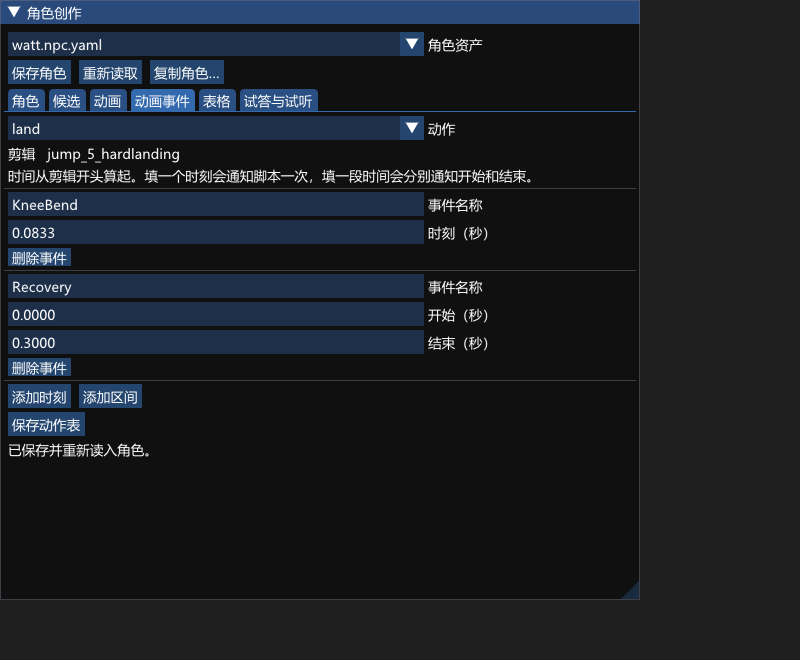
\includegraphics[width=.81\linewidth,trim=0 150 158 0,clip]{../../../output/validation/animation-events/forge-events.png}
\end{center}
\picturecaption{Forge 的角色创作面板，由界面测试运行相同的面板代码并截图。上面是屈膝的时刻，下面是恢复区间。图中已保存 0.30 秒，再次读取后仍显示新值。}

在\button{队友通讯}勾选\button{角色创作}，选中 \code{watt.npc.yaml}，打开\button{动画事件}。在“动作”里选 \code{land}，改完点\button{保存动作表}。编辑器会写入 \code{assets/ai/watt.animator.yaml}。在维修站，玩家和瓦特引用的都是这张表。停止并重新开始游戏后，主角会读取刚保存的时间。

\clearpage
\section*{游戏脚本接收动画事件}

脚本先用 \code{Animator.Bind} 把动作表交给角色。此后调用 \code{Animator.Play(Id, "land", true)}，引擎按名找到模型里的着地剪辑，从头播放。动作表可以共用，两名角色各有自己的播放时间。其中一位提前站起，不会关掉另一位的恢复区间。

\picturecaption{C\# 示例，摘自 \code{SandboxProject/Source/StationMotion.cs} 的 \code{Update}，以下用角色编号 \code{id} 简写。}
\begin{verbatim}
AnimationEvent notice;
while (Animator.TryRead(id, out notice))
{
    if (notice.State == "land" && notice.Name == "Recovery")
        Recovering = notice.Phase == NotifyPhase.Begin;
}
\end{verbatim}

读到 \code{Begin}，恢复开始；读到 \code{End}，恢复结束。这里用循环，是因为画一帧所花的时间有长有短。一帧如果从 0.07 秒跳到 0.22 秒，脚本会先收到 0.0833 秒的屈膝通知，再收到 0.2083 秒的结束通知。脚本读走一条，下一次就读下一条。只需判断某个区间此刻是否开启时，可以直接调用 \code{Animator.IsOpen(id, "Recovery")}。

动作播到一半也可能被替换。假如恢复刚开始就切到待机，脚本仍会收到 \code{End}，其中的 \code{Interrupted} 为真，\code{Seconds} 是切换时动作已播了几秒。将来做连续动作时，可以在第一段剪辑上添加名为 \code{NextInput} 的区间。它开启期间是否接受输入、接着播哪段动作，由游戏脚本决定。

引擎在 \code{AnimationTimeline::Advance} 中比较这次更新前后的剪辑时间。循环动作走到结尾时，先发完本轮最后的事件，再处理下一轮第零秒的事件。实测用两名角色播放同一份动作表，一名播完，一名在第零秒改播待机。前者依次收到恢复开始、屈膝和恢复结束，后者只收到开始和被打断的结束。输出在 \code{output/validation/animation-events/}。

\picturecaption{可对照 Epic 的 \href{https://dev.epicgames.com/documentation/en-us/unreal-engine/animation-notifies-in-unreal-engine}{Animation Notifies} 中的 Notify 与 Notify State。Redflag 提供时刻、区间起止和区间查询，使用秒数在表单中编辑。}
